\documentclass{article}

\usepackage{graphicx}
\usepackage{rotating}
\usepackage{amsmath}
\usepackage{fancyhdr}
\usepackage{listings}
\usepackage{xcolor}
\usepackage{textcomp}
\usepackage{float}
\usepackage[sorting=none]{biblatex}
\usepackage[margin=1in]{geometry}
\usepackage[font={small,it}]{caption}
\usepackage{placeins}
\usepackage{xepersian}

%\DeclareMathOperator*{\btie}{\bowtie}
\addbibresource{bibliography.bib}
\settextfont[Scale=1.2]{B-NAZANIN.TTF}
\setlatintextfont[Scale=1]{Times New Roman}
\renewcommand{\baselinestretch}{1.5}
\pagestyle{fancy}
\fancyhf{}
\rhead{تکلیف چهارم درس پایگاه داده‌ها 1}
\lhead{\thepage}
\rfoot{علیرضا ابره فروش}
\lfoot{9816603}
\renewcommand{\headrulewidth}{1pt}
\renewcommand{\footrulewidth}{1pt}
%%%%%%%%%%
\lstset
{
    language=[latex]tex,
    basicstyle=\ttfamily,
    commentstyle=\color{black},
    columns=fullflexible,
    keepspaces=true,
    upquote=true,
    showstringspaces=false,
    morestring=[s]\\\%,
    stringstyle=\color{black},
}
%%%%%%%%%%

\begin{document}
\begin{titlepage}
\begin{center}

\includegraphics[width=0.4\textwidth]{figures/IUT Logo.png}\\
        
\LARGE
\textbf{دانشگاه صنعتی اصفهان}\\
\textbf{دانشکده مهندسی برق و کامپیوتر}\\
        
\vfill
        
\huge
\textbf{عنوان: تکلیف چهارم درس ریزپردازنده}\\
        
\vfill
        
\LARGE
\textbf{نام و نام خانوادگی: علیرضا ابره فروش}\\
\textbf{شماره دانشجویی: 9816603}\\
\textbf{نیم\,سال تحصیلی: پاییز 1400}\\
\textbf{مدرّس: دکتر عارف کریمی افشار}\\
\end{center}
\end{titlepage}


%\tableofcontents
\newpage


\section{}
مراحل ده‌گانه‌ی طراحی پایگاه داده به شرح زیر است.
\begin{enumerate}
    \item \textbf{\lr{Identify Entities}:}
نقش‌ها، رویدادها، مکان‌ها، اشیاءِ ملموس، یا مفاهیمی که نهایتا کاربر درباره‌ی آن‌ها داده نگه‌داری می‌کند را مشخص کنید.
    \item \textbf{\lr{Find Relationships}:}
وابستگی طبیعی بین هر جفت از \lr{entity}ها را با استفاده از یک ماتریس رابطه پیدا کنید.
	\item \textbf{\lr{Draw Rough ERD}:}
\lr{entity}ها را در مستطیل‌ها و روابط را روی قسمت‌های خطی که \lr{entity}ها را به هم ربط می‌دهند قرار دهید.
	\item \textbf{\lr{Fill in Cardinality}:}
تعداد وقوع یک \lr{entity} را به ازای وقوع یکتای \lr{entity} مربوط به آن تعیین کنید.
	\item \textbf{\lr{Define Primary Keys}:}
\lr{attribute} یا \lr{attribute}هایی که وقوع دقیقا یک رکورد از هر \lr{entity} را مشخص می‌کند را مشخص کنید.
	\item \textbf{\lr{Draw Key-Based ERD}:}
روابطِ \lr{Many-to-Many} را حذف کنید و کلید‌های اصلی و خارجی را در هر \lr{entity} وارد کنید.
	\item \textbf{\lr{Identify Attributes}:}
جزئیات اطلاعاتی(فیلدها) که برای سیستم درحال توسعه الزامی هستند را نام‌گذاری کنید.
	\item \textbf{\lr{Map Attributes}:}
هر \lr{attribute} را با دقیقا یک \lr{entity} که آن را توصیف می‌کند، نظیر کنید.
	\item \textbf{\lr{Draw Fully Attributed ERD}:}
\lr{ERD}ِ گام ششم را با \lr{entity}ها و روابط کشف شده در گام هشتم سازگار کنید.
	\item \textbf{\lr{Check Results}:}
آیا \lr{ERD}ِ نهایی سیستم داده را به دقت مجسم می‌کند؟
\end{enumerate}

\section{}
\subsection{\lr{Composite Attribute}}
برای پیاده‌سازی فیزیکی این نوع \lr{attribute}ها می‌توان هر عنصرِ آن‌ها را در هر \lr{entity} همانند \lr{attribute}های عادیِ آن \lr{entity} به \lr{entity} اضافه می‌کرد. در طراحی برای متمایز کردنشان می‌توان از \lr{indent} استفاده کرد.
\subsection{\lr{Multivalued Attribute}}
برای پیاده‌سازی فیزیکی این نوع \lr{attribute}ها می‌توان یک \lr{table} متناظر با آن \lr{attribute} ایجاد کرد و کلید خارجی از \lr{entity}ی اولیه برای آن تعریف کرد.

\section{}
\lr{weak entity set}، \lr{entity set}ی است که برای تعریف کلید خودش به یک \lr{entity}ی دیگر وابسته است و بدون این کلید خارجی قادر به مشخص کردن هر رکورد به صورت یکتا نیست. \lr{entity set}ی که \lr{weak} نباشد \lr{strong} است. درست است که با این کار پایگاه‌داده‌ی فیزیکی کارش را درست انجام می‌دهد، اما از نظر مدل نتیجه مد نظرمان را نداریم و مفاهیم مورد نظرمان به طور کامل منتقل نمی‌شوند.
\section{}
\subsection{\lr{a}}
\lr{entity}های \lr{Bank Branch}، \lr{Account} و \lr{Loan} موجودیت‌های \lr{weak}، و سایر \lr{entity}ها موجودیت‌های \lr{strong}، هستند.
\subsection{\lr{b}}
\begin{itemize}
    \item [$\bullet$] رابطه‌ی \lr{Branches}:
هر بانک یک تا چند(\lr{N}) شعبه را پوشش‌دهی می‌کند و هر شعبه تحت پوشش دقیقا یک بانک است.
    \item [$\bullet$] رابطه‌ی \lr{Accts}:
هر شعبه صفر تا چند(\lr{N}) حساب را پوشش‌دهی می‌کند و هر حساب تحت پوشش دقیقا یک شعبه است.
    \item [$\bullet$] رابطه‌ی \lr{Loans}:
هر شعبه صفر تا چند(\lr{N}) وام را اعطا می‌کند و هر وام توسط دقیقا یک شعبه اعطا می‌شود.
    \item [$\bullet$] رابطه‌ی \lr{A-C}:
هر حساب متعلق به یک تا چند(\lr{N}) مشتری است و هر مشتری دارای یک تا چند(\lr{M}) حساب است.
    \item [$\bullet$] رابطه‌ی \lr{L-C}:
هر وام می‌تواند به یک تا چند(\lr{N}) مشتری اعطا شود و هر مشتری می‌تواند صفر تا چند(\lr{M}) وام بگیرد.

\end{itemize}
\subsection{\lr{c}}
\begin{itemize}
    \item [$\bullet$] لیست مشخصات مشتری‌هایی که مانده حساب بیشتر از 1 میلیون دارند
    \item [$\bullet$] مجموع مبلغ وام‌های داده شده توسط یک شعبه خاص
    \item [$\bullet$] تعداد حساب‌های یک مشتری خاص
\end{itemize}
\subsection{\lr{d}}
به ترتیب:
\begin{itemize}
    \item [$\bullet$] فیلدهای \lr{Customer} از \lr{inner join}ِ \lr{Customer} و \lr{A-C} و \lr{Account} به شرط یکسان بودن \lr{SSN}ها در \lr{Customer} و \lr{A-C}، و \lr{AccNo}ها در \lr{A-C} و \lr{Account} و مجموع \lr{Balance}های بیشتر از 1 میلیون به تفکیک \lr{SSN}ها.
    \item [$\bullet$] مجموع روی فیلد \lr{Amount} از \lr{inner join}ِ \lr{Loan} و \lr{Loans} و \lr{Bank Branch} به شرط یکسان بودن \lr{LoanNo}ها در \lr{Loan} و \lr{Loans}، و \lr{BrNo}ها در \lr{Loans} و \lr{Bank Branch} به تفکیک \lr{BrNo}.
    \item [$\bullet$] شمارش روی رکوردهای \lr{A-C} به تفکیک \lr{SSN}.
\end{itemize}
\subsection{\lr{e}}
اضافه کردن \lr{attribute} به نام \lr{sponsor\_ssn} در \lr{entity}ی \lr{Loan} که کلید خارجی از \lr{entity}ی \lr{Customer} است.

\section{}
\subsection{\lr{a}}
%begintable
\begin{table}[H]
\resizebox{\textwidth}{!}{%
\begin{tabular}{|c|c|c|c|c|c|c|c|c|c|c|c|}
\hline
                           & \textbf{\lr{Branch}} & \textbf{\lr{Manager}} & \textbf{\lr{Provider}} & \textbf{\lr{Staff}} & \textbf{\lr{Time}} & \textbf{\lr{Food}}  & \textbf{\lr{Organization}} & \textbf{\lr{Complaint}} & \textbf{\lr{Customer}}     & \textbf{\lr{Ingredient}} \\
\hline\textbf{\lr{Branch}}       &                      & \lr{Managed by}       & \lr{Supplied by}       & \lr{Employes}       &                    &                     & \lr{Caters}                & \lr{Has}                &                            &                          \\
\hline\textbf{\lr{Manager}}      & \lr{Manages}         & \lr{Superior to}      &                        &                     &                    &                     &                            &                         &                            &                          \\
\hline\textbf{\lr{Provider}}     & \lr{Supplies}        &                       &                        &                     &                    &                     &                            &                         &                            & \lr{Provides}   \\
\hline\textbf{\lr{Staff}}        & \lr{Employed by}     &                       &                        &                     & \lr{Works in}      &                     &                            &                         &                            &                          \\
\hline\textbf{\lr{Time}}         &                      &                       &                        & \lr{Is assigned to} &                    &                     &                            &                         &                            &                          \\
\hline\textbf{\lr{Food}}         &                      &                       &                        &                     &                    &                     &                            &                         & \lr{Ordered by, Graded by} & \lr{Is made of}          \\
\hline\textbf{\lr{Organization}} & \lr{Catered by}      &                       &                        &                     &                    &                     &                            &                         &                            &                          \\
\hline\textbf{\lr{Complaint}}    & \lr{Assigned to}     &                       &                        &                     &                    &                     &                            &                         & \lr{Installed by}          &                          \\
\hline\textbf{\lr{Customer}}     &                      &                       &                        &                     &                    & \lr{Orders, Grades} &                            & \lr{Installs}           &                            &                          \\
\hline\textbf{\lr{Ingredient}}   &                      &                       & \lr{Provided by}       &                     &                    & \lr{Make}           &                            &                         &                            &                         
\end{tabular}%
}
\end{table}
%endtable

\subsection{\lr{b}}
\begin{itemize}
    \item [$\bullet$] نام شعبه در در سفارشات و غذاها مشخص نمی‌شود.
    \item [$\bullet$] هر تامین‌کننده می‌تواند با صفر تا چند شعبه کار کند.
    \item [$\bullet$] هر سازمان دقیقا با یک شعبه قرارداد دارد.
    \item [$\bullet$] به هر مشتری صرف نظر از اینکه مشترک هست یا موردی یک شناسه اختصاص می‌دهیم.
    \item [$\bullet$] اینکه شکایت مربوط به چه سرویسی یا چه غذایی است لحاظ نمی‌شود.
    \item [$\bullet$] هر مشتری تنها پس از صرف غذا نمره می‌دهد و نمره‌دهی بدون صرف غذا نداریم.
\end{itemize}
\begin{figure}[H]
    \centering
    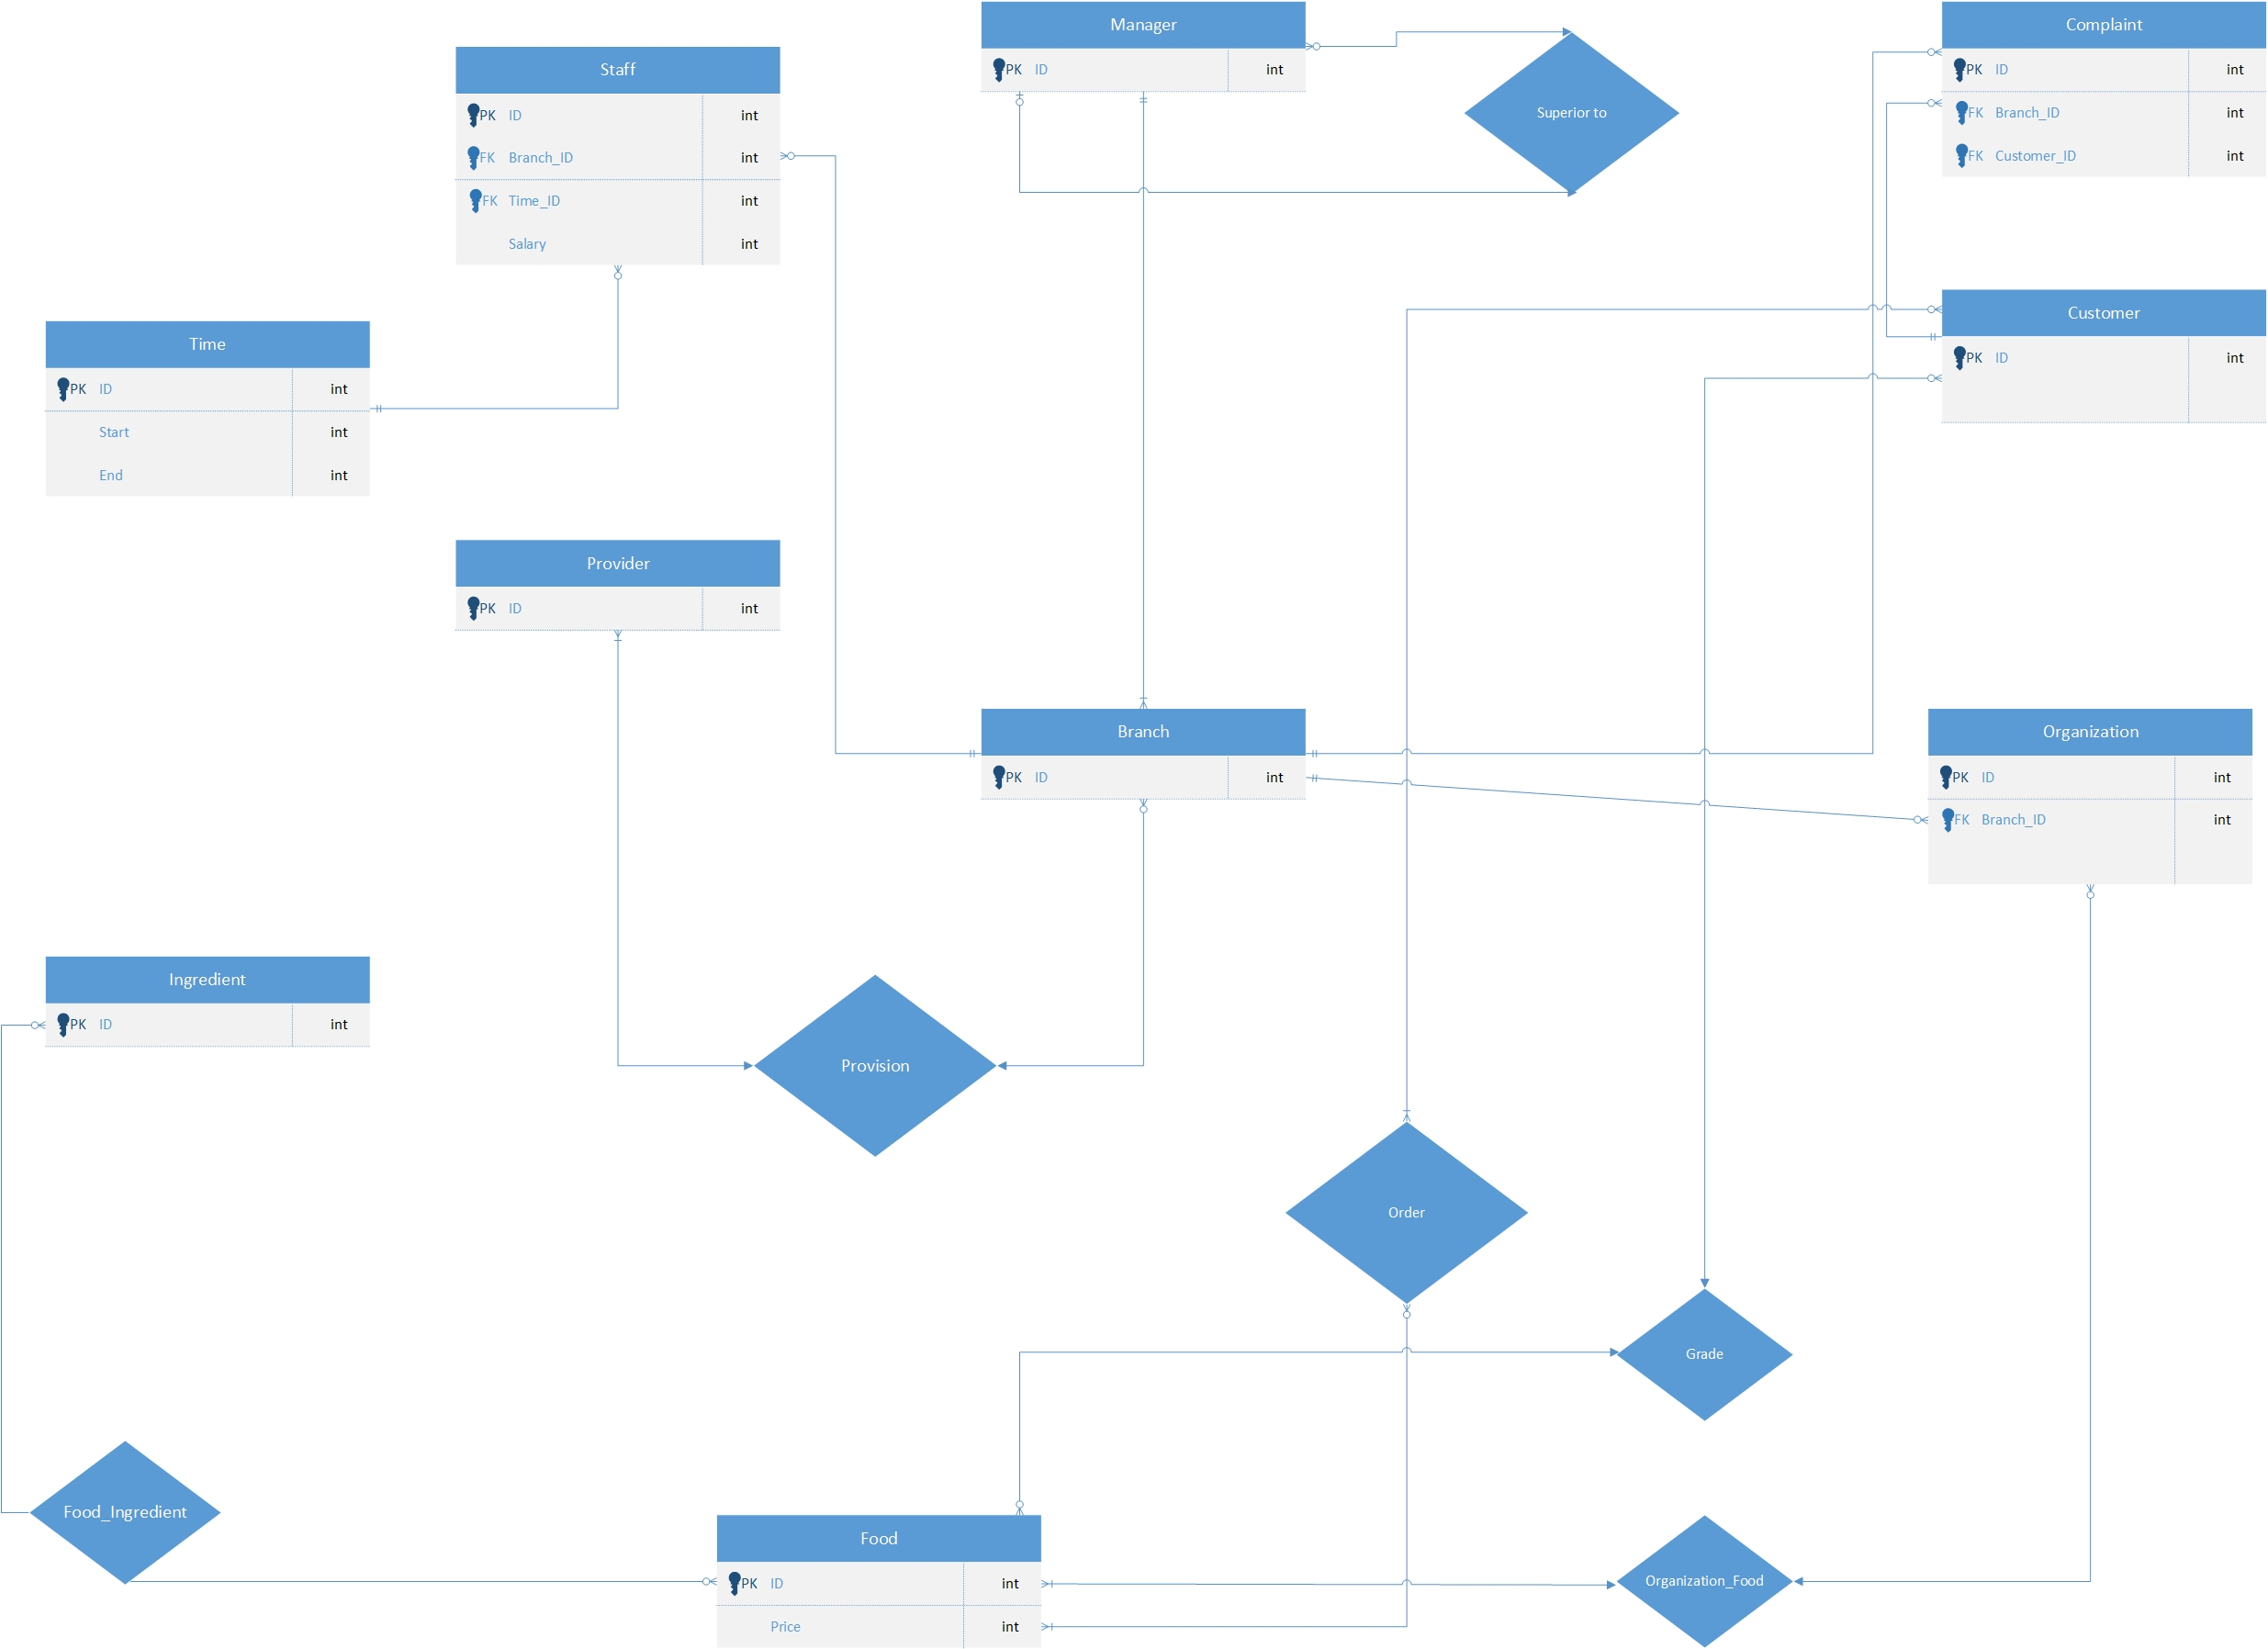
\includegraphics[width=1\textwidth]{figures/D1.jpg}
    \caption
	{
\lr{4-a}
	}
    \label{fig:fig1}
\end{figure}

\subsection{\lr{b}}
\begin{figure}[H]
    \centering
    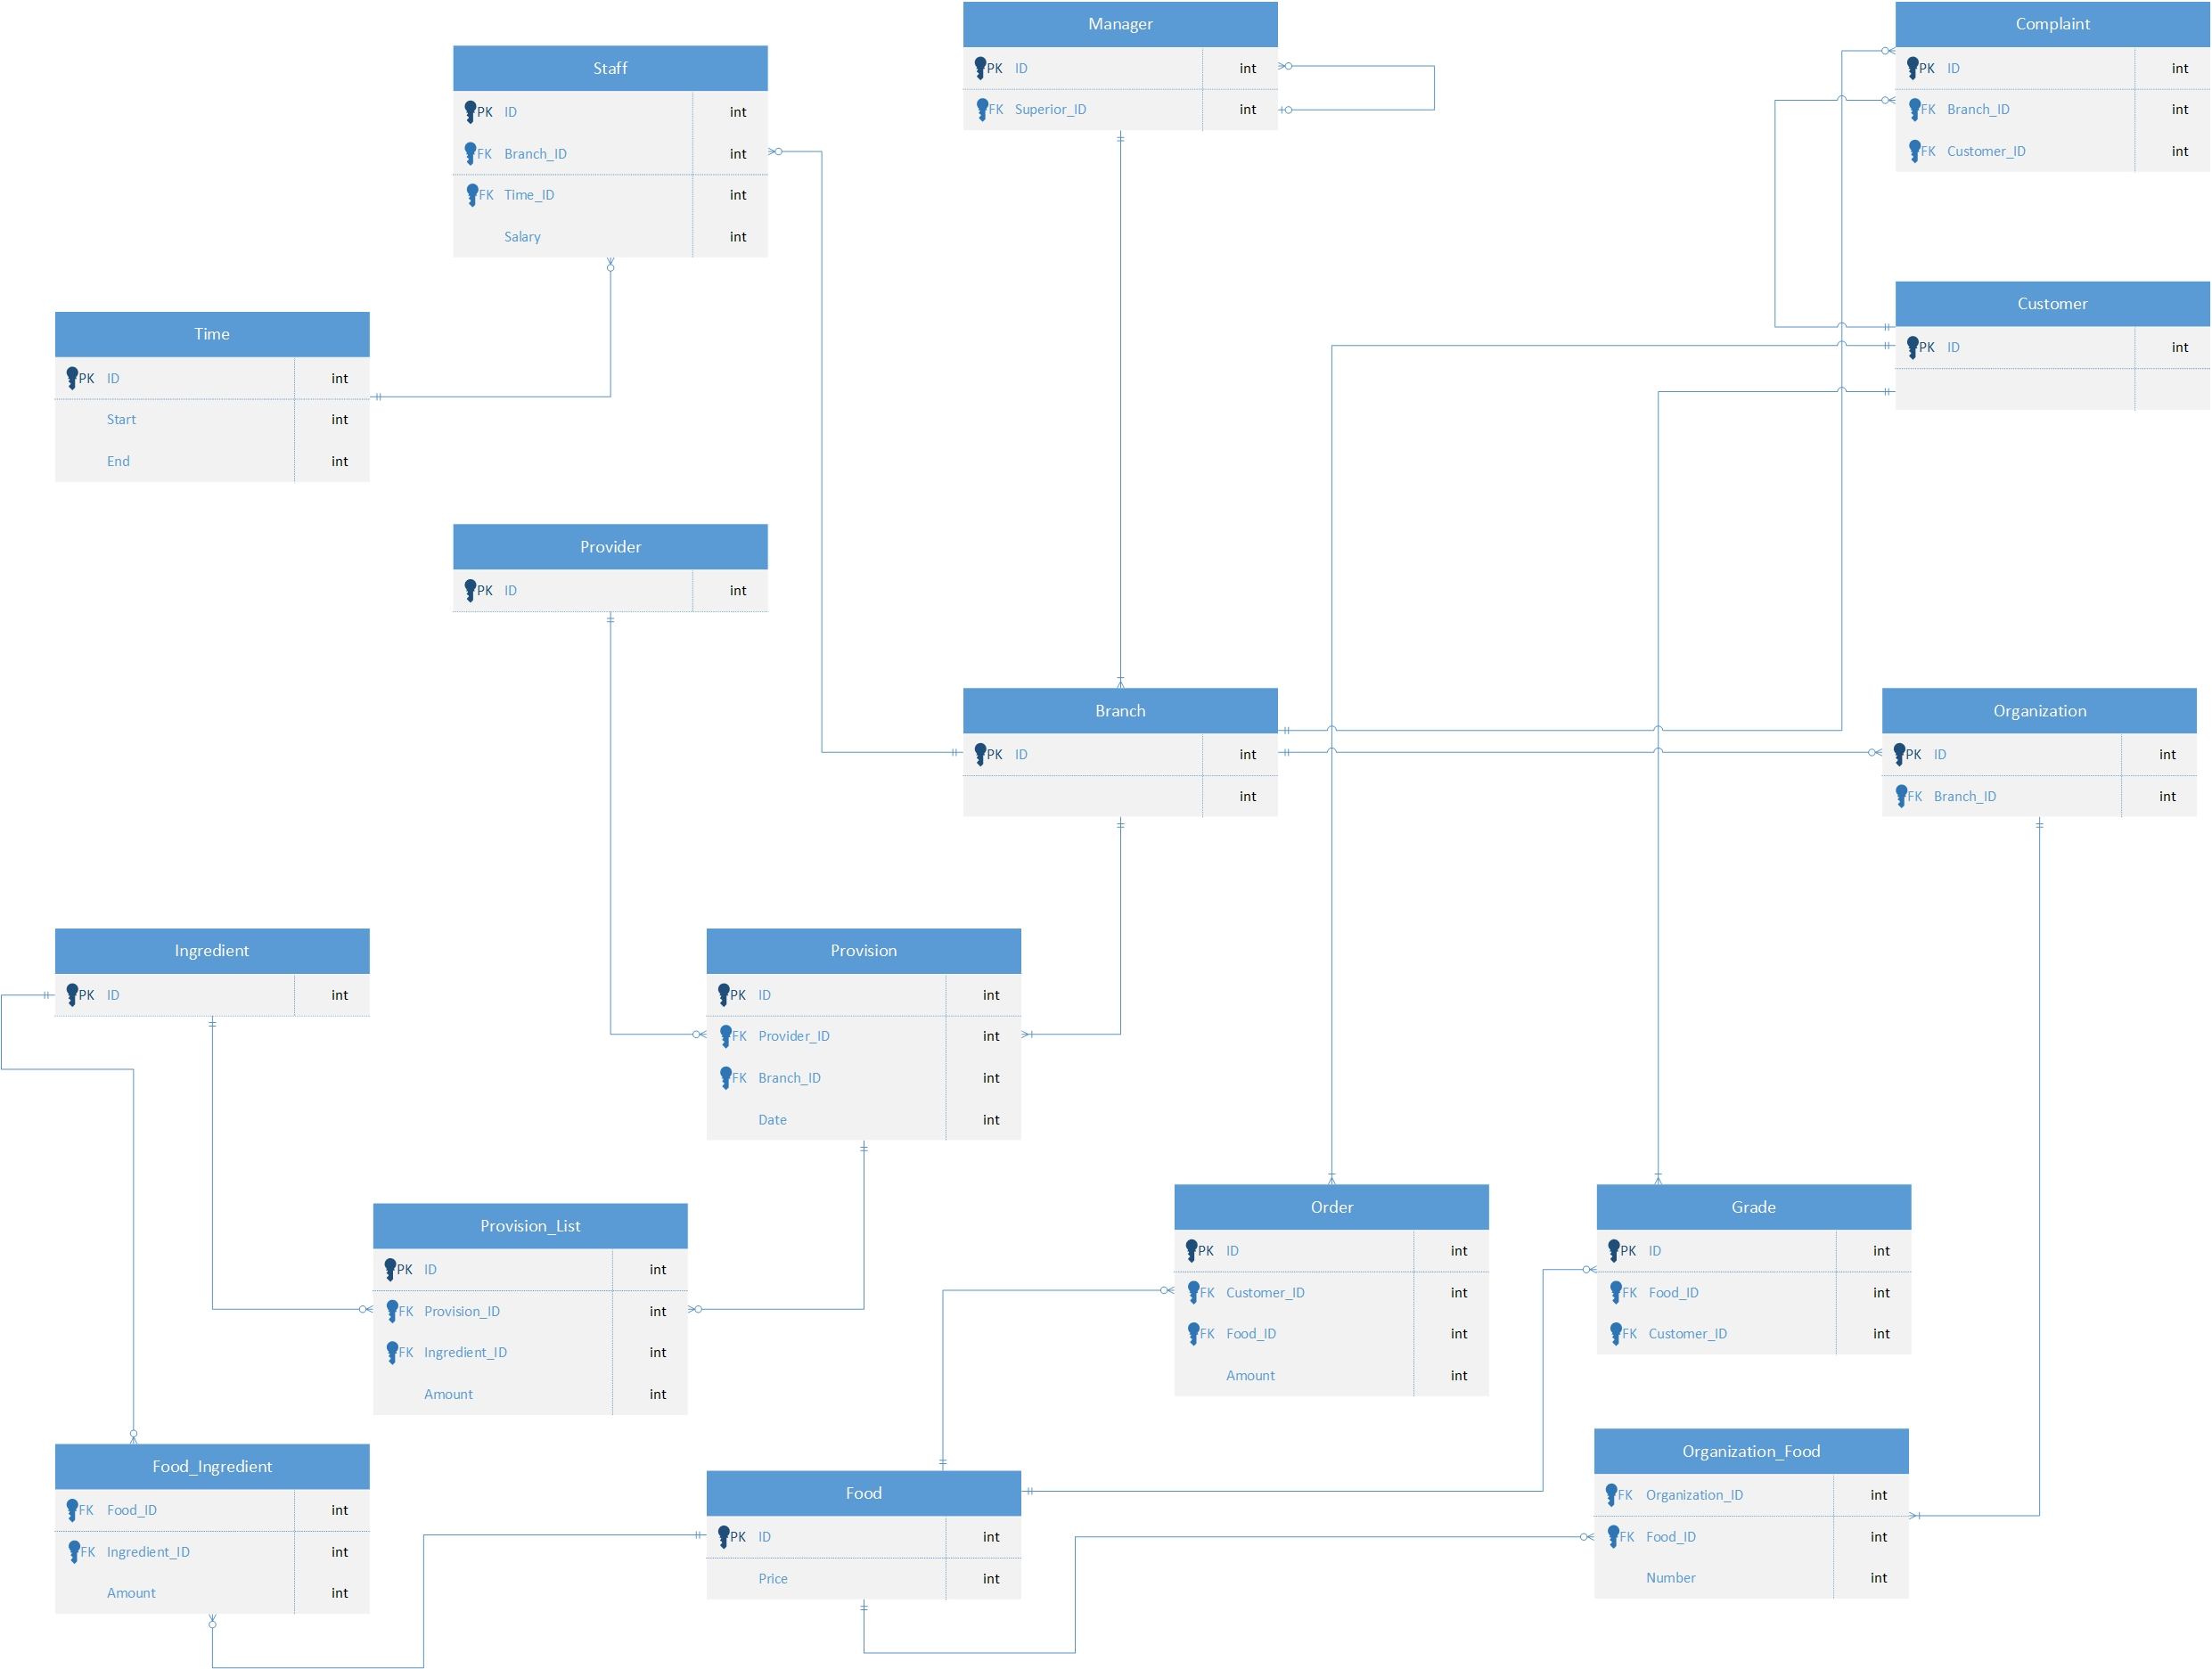
\includegraphics[width=1\textwidth]{figures/D2.jpg}
    \caption
	{
\lr{4-b}
	}
    \label{fig:fig1}
\end{figure}

\section{}
\begin{itemize}
    \item [$\bullet$] هر \lr{Reservation} متعلق به دقیقا یک مشتری است.
    \item [$\bullet$] کاردینالیتی‌های بیشتر از 1 به \lr{Many} نظیر شده اند.
\end{itemize}

%beigintable
\begin{table}[H]
\resizebox{\textwidth}{!}
{
\begin{tabular}{|c|c|c|c|c|c|c|c|c|}
\hline                          & \textbf{\lr{Customer}} & \textbf{\lr{Reservation}} & \textbf{\lr{Flight}} & \textbf{\lr{Stewardess}} & \textbf{\lr{Pilot}} & \textbf{\lr{Airport}} & \textbf{\lr{City}} \\
\hline\textbf{\lr{Customer}}    &                        & \lr{Reserves}             &                      &                          &                     &                       &                    \\
\hline\textbf{\lr{Reservation}} & \lr{Reserved by}       &                           & \lr{Services}        &                          &                     &                       &                    \\
\hline\textbf{\lr{Flight}}      &                        & \lr{Is the service of}    &                      & \lr{Has}                 & \lr{Has}            & \lr{From, To}         & \lr{From, To}      \\
\hline\textbf{\lr{Stewardess}}  &                        &                           & \lr{Attends at}      &                          &                     & \lr{Works at}         &                    \\
\hline\textbf{\lr{Pilot}}       &                        &                           & \lr{Attends at}      &                          &                     & \lr{Works at}         &                    \\
\hline\textbf{\lr{Airport}}     &                        &                           &                      & \lr{Works with}          & \lr{Works with}     &                       & \lr{Is located in} \\
\hline\textbf{\lr{City}}        &                        &                           &                      &                          &                     & \lr{Has}              &                   
\end{tabular}%
}
\end{table}
%endtable
%%%%%%%%%%%%%%%%%%%%%%%%%%%%%%%%%%%
\begin{figure}[H]
    \centering
    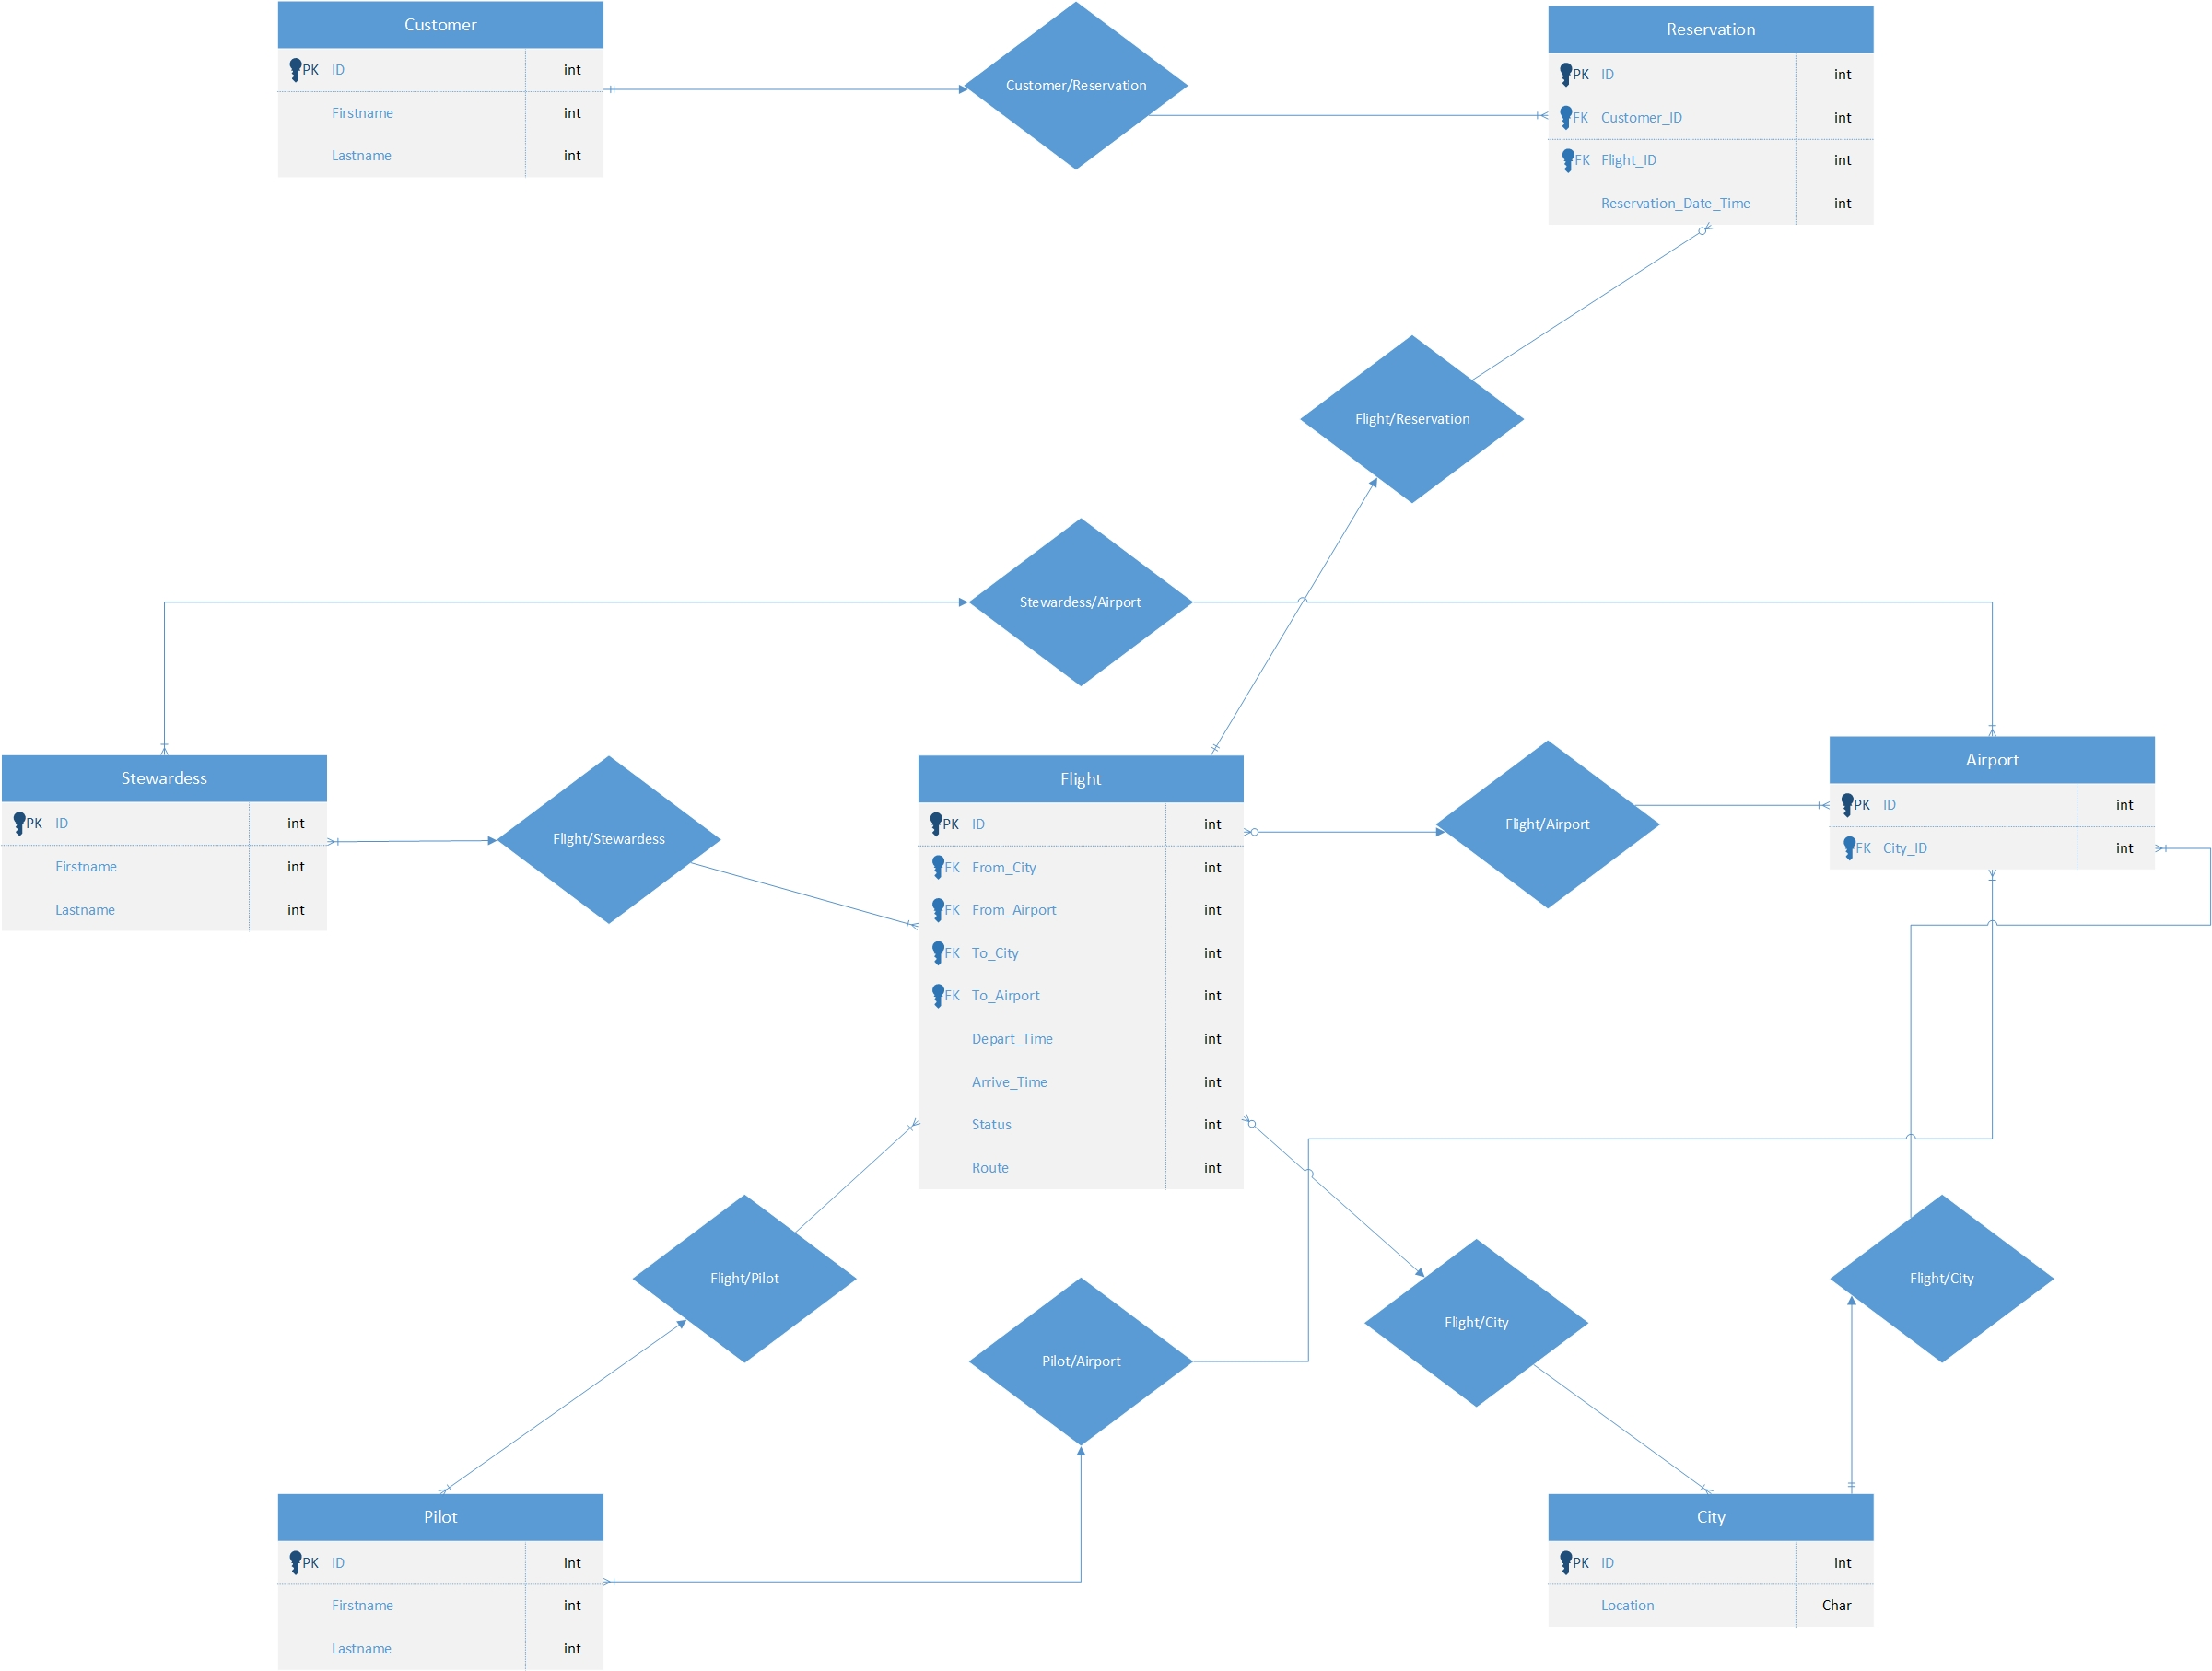
\includegraphics[width=1\textwidth]{figures/D3.jpg}
    \caption
	{
\lr{6-a}
	}
    \label{fig:fig1}
\end{figure}
\begin{figure}[H]
    \centering
    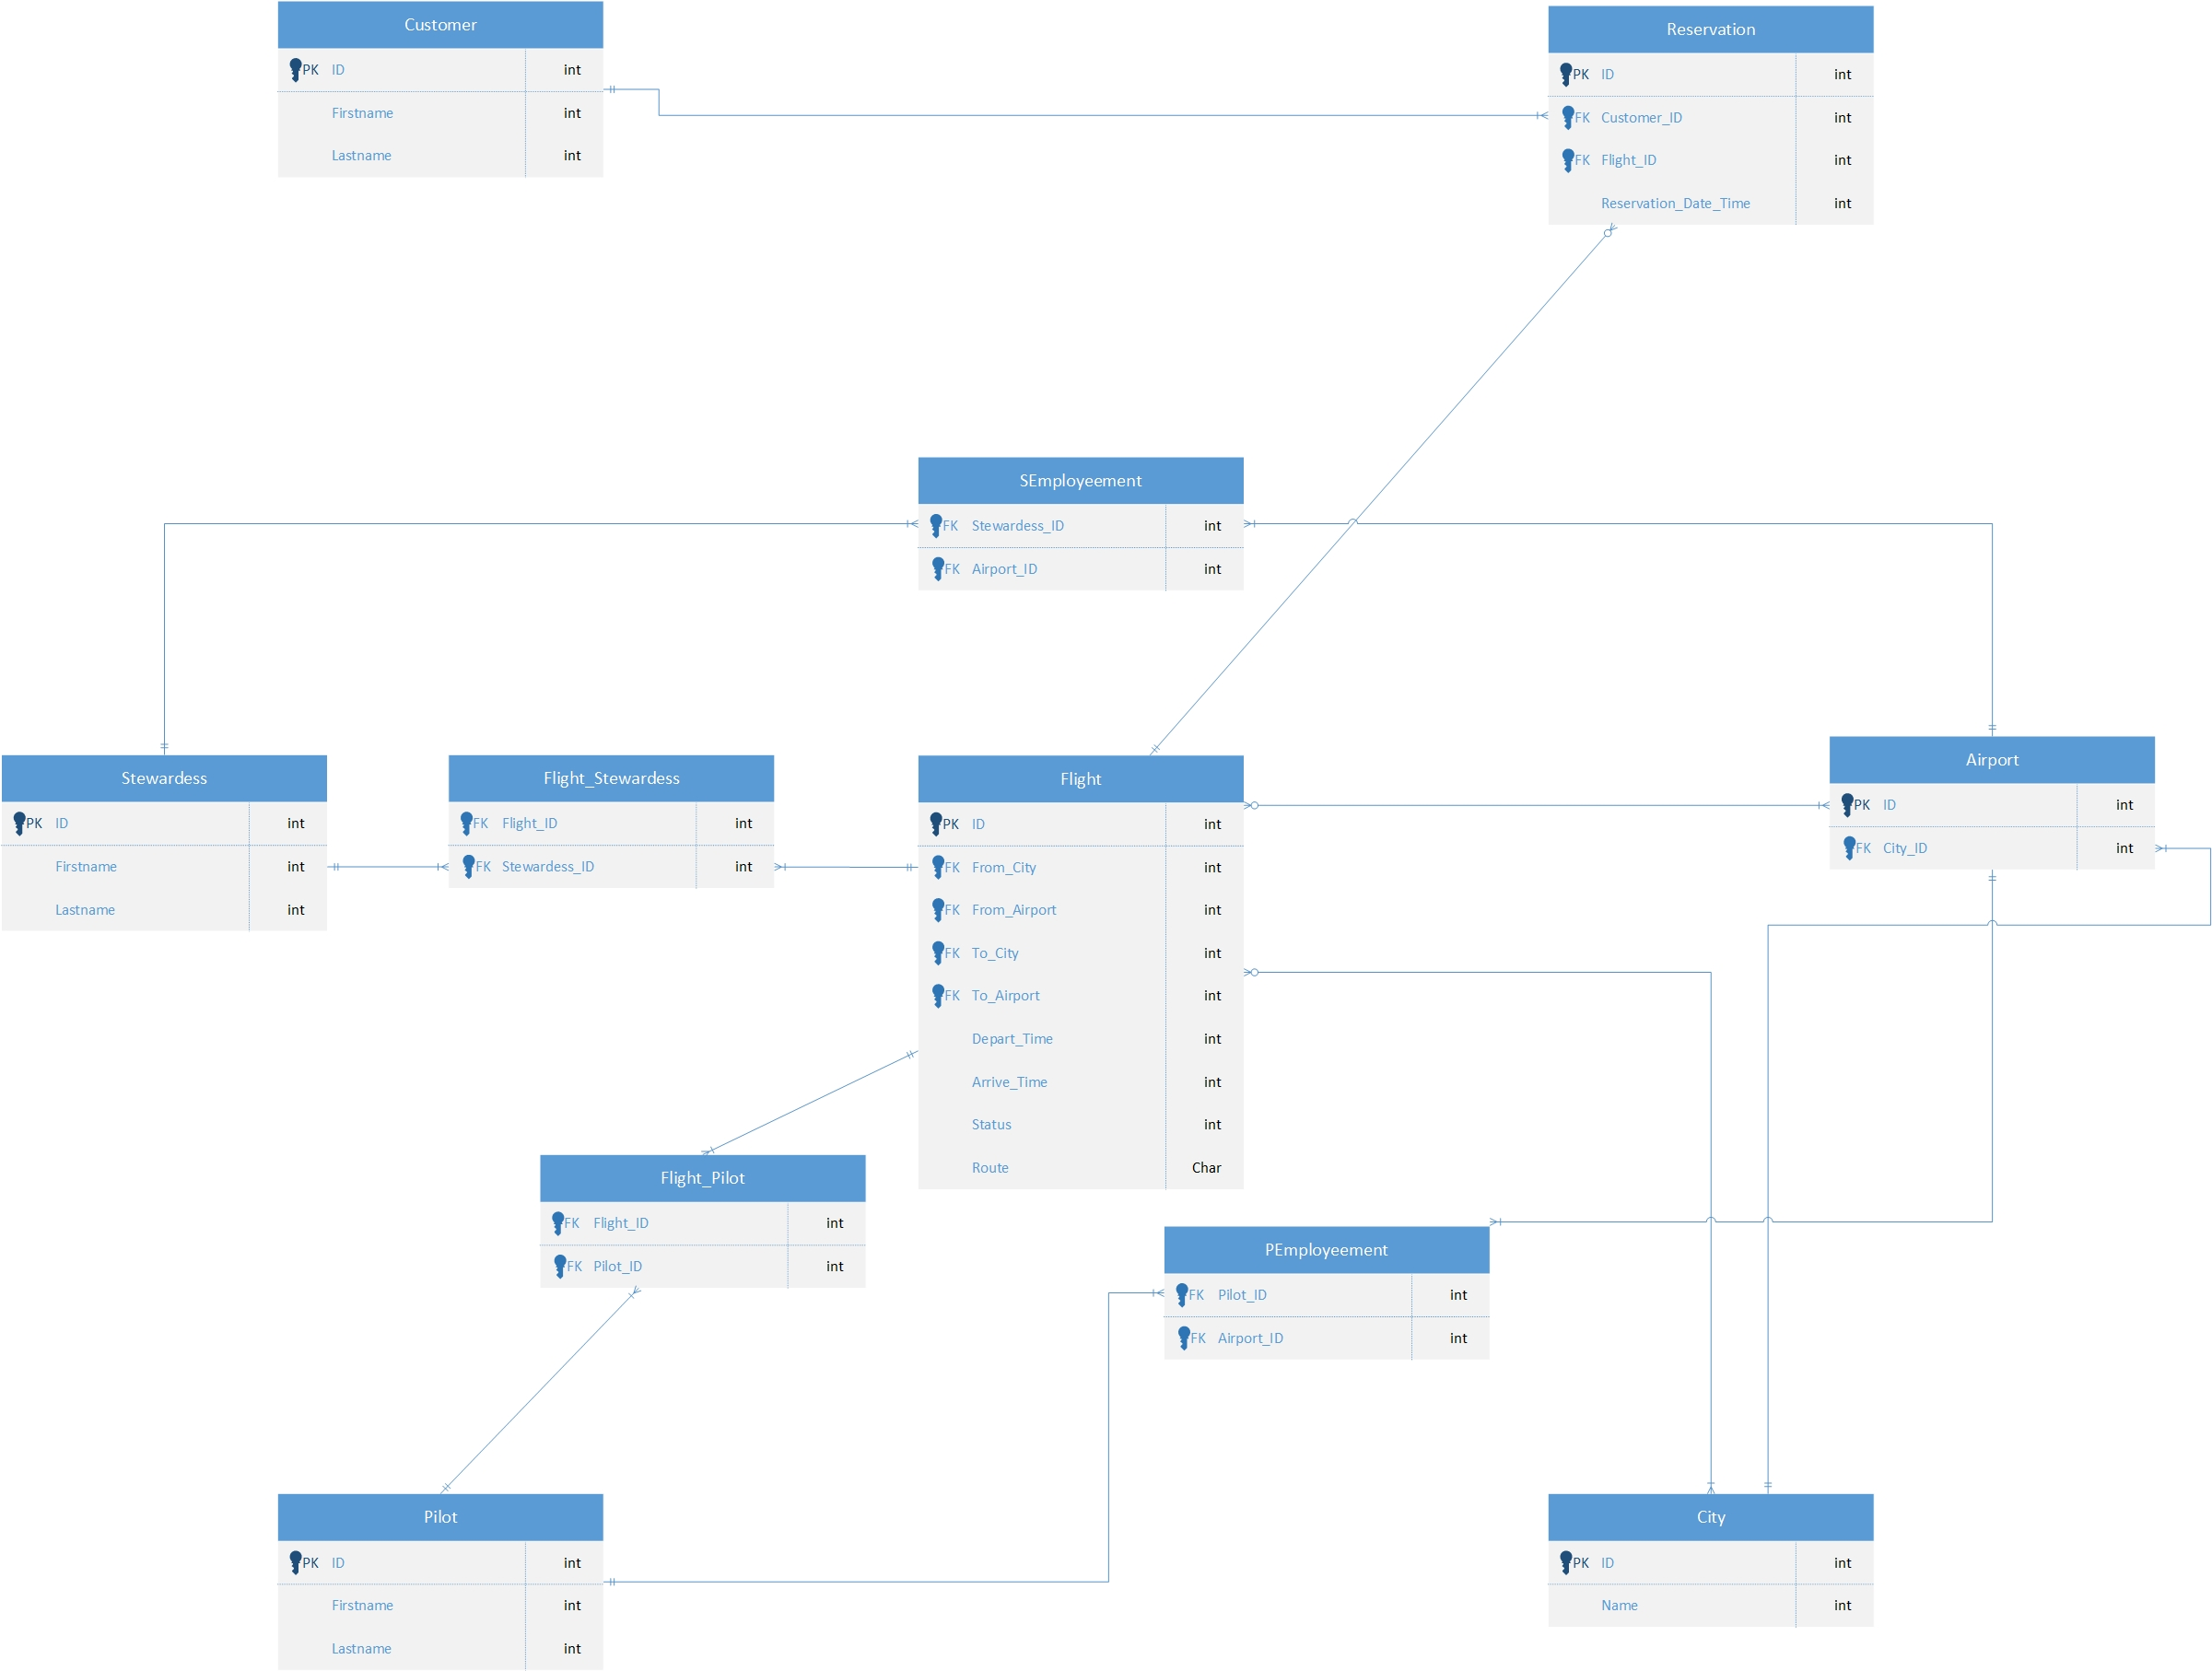
\includegraphics[width=1\textwidth]{figures/D4.jpg}
    \caption
	{
\lr{6-b}
	}
    \label{fig:fig1}
\end{figure}
\begin{itemize}
    \item [$\bullet$] درصورت عدم وضوح کافی تصاویر، فایلِ \lr{Visio}ی دیاگرام‌ها در فایل زیپ موجود است.
\end{itemize}

\section{}
\subsection{\lr{a}}
داخل فایل \lr{SQL}
\subsection{\lr{b}}
داخل فایل \lr{SQL}
%------------------------------------------------------------------------------------------


\section*{منابع}
\renewcommand{\section}[2]{}%
\begin{thebibliography}{99} % assumes less than 100 references
%چنانچه مرجع فارسی نیز داشته باشید باید دستور فوق را فعال کنید و مراجع فارسی خود را بعد از این دستور وارد کنید


\begin{LTRitems}

\resetlatinfont

\bibitem{b1} None
\end{LTRitems}

\end{thebibliography}


\end{document}
